\documentclass[mathserif,utf8,xcolor=table,10pt]{beamer}

\usepackage[T2A]{fontenc}
\usepackage[utf8]{inputenc}
\usepackage[english,russian]{babel}
\usepackage{graphicx}
\usepackage{ulem}
\usepackage{textpos}
\usepackage{hyperref}
%\usepackage{listings}
\usepackage{listingsutf8}
%\usepackage{minted}
\usepackage{tikz}
\usetikzlibrary{mindmap,shadows}
%\usepackage[hidelinks,pdfencoding=auto]{hyperref}


\definecolor{dkgreen}{rgb}{0,0.6,0}
\definecolor{gray}{rgb}{0.5,0.5,0.5}
\definecolor{mauve}{rgb}{0.58,0,0.82}

\lstset{frame=tb,
  language=C++,
%  aboveskip=3mm,
%  belowskip=3mm,
  showstringspaces=false,
  columns=flexible,
  basicstyle={\scriptsize\ttfamily},
  numbers=none,
  numberstyle=\tiny\color{gray},
  keywordstyle=\color{blue},
  commentstyle=\color{dkgreen},
  stringstyle=\color{mauve},
  breaklines=true,
%  breakatwhitespace=true,
  tabsize=2,
 % escapeinside={\%*}{*)},
 % inputencoding=utf8,
  inputencoding=utf8/utf8,
  texcl=true,
}

\mode<presentation>
{
        \usetheme{Antibes}
        \setbeamercovered{transparent}
}

\title{Введение в С/C++: структура программ, переменные, выражения, операторы}
\institute{Степулёнок Денис Олегович}
\date[октябрь 2015]{14 октября 2015 года}
\subject{Занятие 1}

\newcommand{\hl}{\only{\cellcolor{yellow}}}
\renewcommand{\le}{\leqslant}
\renewcommand{\ge}{\geqslant}
\setlength{\arrayrulewidth}{1pt}

\begin{document}

%\begin{frame}
%\titlepage
%\end{frame}


% Языки высокого и низкого уровня. Позиционирование языка C. Преимущества и недостатки C.
\section{Языки высокого и низкого уровня}
\subsection{Уровень языка программирования (ЯП)}

\begin{frame}[t]{Уровень языка программирования (ЯП)}
  \begin{itemize}
    \item \textbf{Высокоуровневый ЯП} --- \textbf{скорость} и \textbf{удобство} разработки (удобство программиста) в том числе за счёт снижения 
    эффективности использования памяти и процессорного времени. 
    Ближе к естественному языку.

    \item \textbf{Язык низкого уровня} --- близок к программированию в машинных кодах (или на ассемблере)
      используемого реального или виртуального (Java, .NET) процессора
  \end{itemize}
\end{frame}

\subsection{Особенности языков высокого уровня}

\begin{frame}[t]{Язык высокого уровня}

   Основная черта - \textbf{абстракция}, то есть введение смысловых конструкций, 
   кратко описывающих такие структуры данных и операции над ними, 
   описания которых в машинном коде (или низкоуровневом ЯП) длинны и сложны для понимания.

\end{frame}

\begin{frame}[t]{Основные <<+>> ЯП низкого уровня}
  \begin{itemize}
    \item эффективное использование процессорного $t$ и памяти.
    \item часто язык низкого уровня позволяет обратиться к ресурсам, недоступным из языка высокого уровня.
    \item размер исполняемого файла готовой программы получается, как правило, меньше.
  \end{itemize}
\end{frame}


\begin{frame}[t]{История языка C}

  C (Си) --- компилируемый статически типизированный ЯП общего назначения,
  разработанный в 1969-1973 годах сотрудником Bell Labs Деннисом Ритчи как развитие языка B.



\end{frame}

\begin{frame}[t]{Возникновение названия языка C}

  \begin{itemize}
  \item 1964 - \textbf{APL} - назван по книге \textbf{A Programming Language} --- ЯП, 
     оптимизированный для работы с массивами, предшественник современных вычислительных сред (MATLAB), 
   использует функциональную парадигму программирования.    
   Разработан Кеном Айверсоном, преподававшим тогда в Гарвардском университете, 
   в качестве системы обозначений для описания вычислений. 
   В 1957 вышла его книга <<A Program Language>>, в которой был описан \textbf{APL}. 
   
\item 1966 - \textbf{BCPL} (Basic Combined Programming Language) --- ЯП,
разработанный Мартином Ричардсом, в Кембриджском университете. 
Изначально предназначался для написания компиляторов для других языков.
  Сейчас BCPL практически не используется, но в своё время он был очень важен из-за хорошей портируемости. 
  Урезанная версия языка с несколько изменённым синтаксисом стала ЯП \textbf{B}, который оказал сильное влияние на \textbf{C}. 
  \end{itemize}
\end{frame}

\begin{frame}[t]{Возникновение названия языка C - 2}
  \begin{itemize}
  
  \item 1969 - Язык \textbf{B} --- интерпретируемый ЯП, разработанный в AT\&T Bell Telephone Laboratories. 
    Является потомком языка BCPL и непосредственным предшественником \textbf{C}. 
    \textbf{B} был в основном произведением Кена Томпсона при содействии Денниса Ритчи и был опубликован в 1969 году.
    
  \item 1972 - \textbf{C} --- название языка является третьей буквой алфавита (намекает что \textbf{C} более совершеннный чем \textbf{B})
  
Успех \textbf{C} в основном связан с тем, что на нём была написана значительная часть операционной системы UNIX, 
которая в итоге приобрела очень большую популярность. 
В связи с её распространённостю, и с тем, что объём ОС измеряется в миллионах строк кода 
(для примера, в последних версиях Linux содержится более 10000000 строк кода), 
задача о переписывании UNIX на другой язык становиться практически невыполнимой 
(также следует учитывать тот факт, что при ручном переписывании неизбежно возникнут ошибки, 
что существенно снизит стабильность работы, а при переводе с использованием программных средств пострадает производительность кода).
Кроме того, \textbf{C}, будучи приближённым к аппаратной реализации компьютера позволяет выжать из него намного больше, 
чем многие другие языки программирования. 
Это обстоятельство показывает бессмысленность перевода UNIX на другой язык. 
Таким образом, если другие языки программирования могут исчезнуть с течением времени, уступив дорогу новым технологиям, 
то \textbf{C} будет жить, пока живёт UNIX. То есть пока существуют компьютеры в том виде, в котором мы их себе представляем.

Первая книга, посвящённая \textbf{C} была написана Керниганом и Ритчи в 1978 году и вышла в свет под названием 
<<Язык программирования Си>>. Эта книга, в среде программистов более известная как <<K\&R>>, стала неофициальным стандартом \textbf{C}.  



  \end{itemize}

\end{frame}


\begin{frame}[t]{C11}

  8 декабря 2011 опубликован новый стандарт для языка С (ISO/IEC 9899:2011)

\end{frame}

% История создания языка C, история C++. Перспективы - язык D
\section{Язык D - http://dlang.org}
\subsection{Язык D}

\begin{frame}[t,fragile]{Развитие C - язык D - http://dlang.org}
  \textbf{D} - объектно-ориентированный, императивный, мультипарадигмальный язык программирования, 
  созданный Уолтером Брайтом из компании Digital Mars. 
  Изначально был задуман как реинжиниринг языка C++, однако, несмотря на значительное влияние С++, не является его вариантом. 
  В D были заново реализованы некоторые свойства C++, 
  также язык испытал влияние концепций из других языков программирования, таких как Java, Python, Ruby, C\# и Eiffel.

\begin{lstlisting}
void main() {
  // Define an array of numbers, double[].
  auto arr = [ 1, 2, 3.14, 5.1, 6 ];
  auto dictionary = [ "one" : 1, "two" : 2, "three" : 3 ];
  // Calls the min function defined below
  auto x = min(arr[0], dictionary["two"]);
}
// Type deduction works for function results
auto min(T1, T2)(T1 lhs, T2 rhs) {
  return rhs < lhs ? rhs : lhs;
}
\end{lstlisting}


\end{frame}

% Установка и настройка IDE Code::Blocks. Запуск программы. Отладка. Решение проблем с настройкой. 
\section{Скачивание, установка, запуск и настройка IDE Code::Blocks}

\subsection{Скачивание с http://www.codeblocks.org/downloads}

\begin{frame}[t]{Code::Blocks --- С/C++ IDE}


\includegraphics[width=0.2\textwidth]{logo}

\url{http://www.codeblocks.org} --- сайт Code::Blocks

\url{http://www.codeblocks.org/downloads/26} скачать:

  \begin{itemize}
    \item \textbf{codeblocks-13.12-setup.exe} - только среда разработки без компилятора и отладчика. 
    \item \textbf{codeblocks-13.12mingw-setup.exe} - IDE + MinGW (компилятор + отладчик).
    \item \textbf{codeblocks-13.12mingw-setup-TDM-GCC-481.exe} - IDE + Альтернативный компилятор и отладчик (TDM).
  \end{itemize}

  Выбирайте: \textbf{codeblocks-13.12mingw-setup.exe}

\end{frame}

\subsection{Установка Code::Blocks}

\begin{frame}[t]{Next > Next > Next}
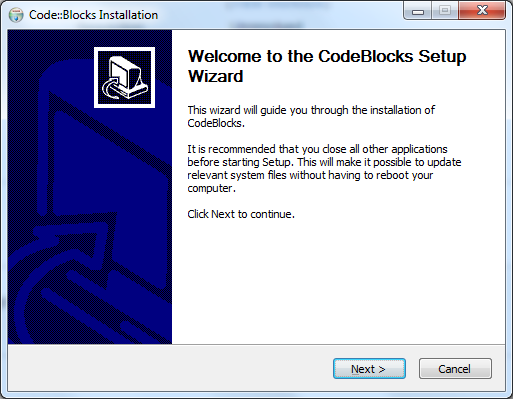
\includegraphics[width=0.5\textwidth]{00_codeblocks/step1.png}
\end{frame}

\begin{frame}[t]{GNU General Public License}
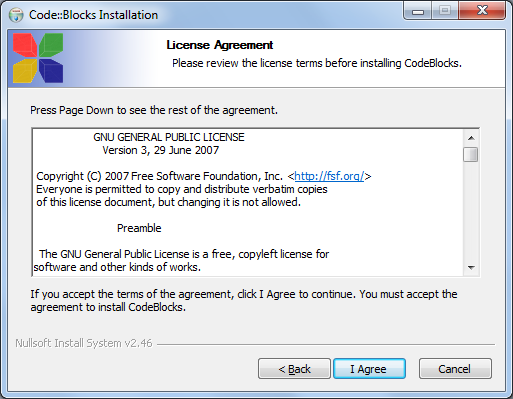
\includegraphics[width=0.5\textwidth]{00_codeblocks/step2.png}
\end{frame}

\subsection{Запуск Code::Blocks}

\begin{frame}[t]{Начальный экран Code::Blocks}
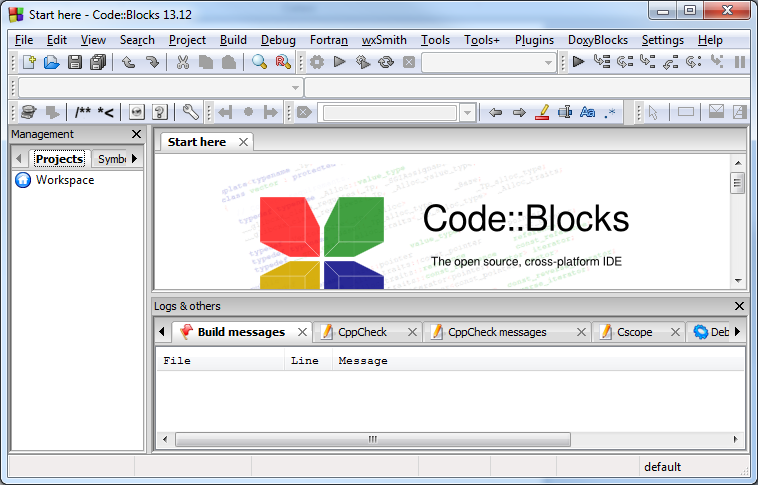
\includegraphics[width=0.7\textwidth]{00_codeblocks/CodeBlocks.png}
\end{frame}

\subsection{Настройка Code::Blocks}

\begin{frame}[t]{Настройки компиляторов для Code::Blocks}
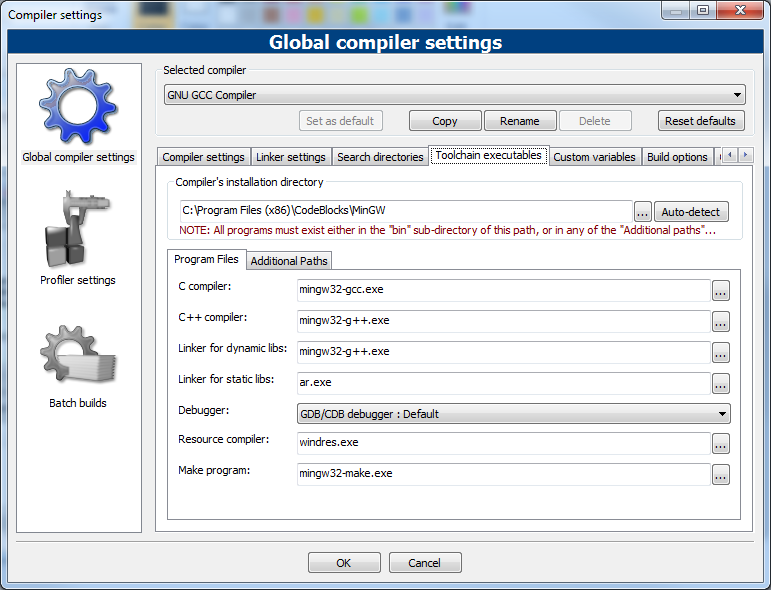
\includegraphics[width=\textwidth]{00_codeblocks/CodeBlocks_GlobalCompilerSettings.png}
\end{frame}

\subsection{Создание проекта в Code::Blocks}

\begin{frame}[t]{Начальный экран Code::Blocks}
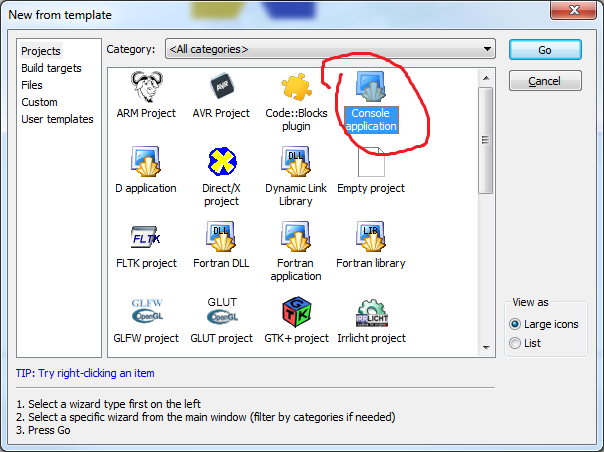
\includegraphics[width=\textwidth]{00_codeblocks/CodeBlocks_Console_application.png}
\end{frame}

\begin{frame}[t]{Выбираем язык программирования C или C++}
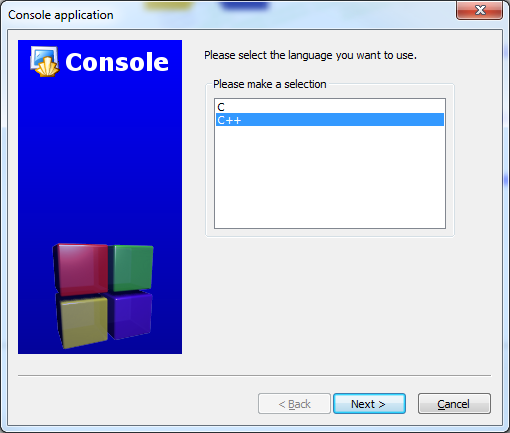
\includegraphics[width=\textwidth]{00_codeblocks/CodeBlocks_cpp.png}
\end{frame}

\subsection{Горячие клавиши / Hot Keys / Shortcuts}

\begin{frame}[t]{Горячие клавиши / Hot Keys / Shortcuts}
  Редактор:
  \begin{itemize}
    \item \textbf{Ctrl + Z} --- Отменить последнее действие. 
    \item \textbf{Ctrl + Shift + Z} --- Redo last action. 
    \item \textbf{Ctrl + X} --- Вырезать выделенный текст. 
    \item \textbf{Ctrl + C} --- Скопировать текст. 
    \item \textbf{Ctrl + V} --- Вставить текст. 
    \item \textbf{Ctrl + A} --- Выделить весь текст. 
    \item \textbf{F11} --- Переключение header / source. 
    \item \textbf{Ctrl + Shift + C} --- Закомментировать выделенный код. 
    \item \textbf{Ctrl + Shift + X} --- Раскомментировать выделенный код. 
    \item \textbf{Ctrl + Пробел} --- Автодополнение. 
    \item \textbf{Ctrl + B} --- Поставить закладку. 
    \item \textbf{Alt + PgUp} / \textbf{Alt + PgDown} --- Ходить по закладкам. 
  \end{itemize}
\end{frame}

\begin{frame}[t]{Горячие клавиши / Hot Keys / Shortcuts}
  Работа с файлами:
  \begin{itemize}
    \item \textbf{Ctrl + N} --- Новый файл или проект. 
    \item \textbf{Ctrl + O} --- Открыть файл или проект. 
    \item \textbf{Ctrl + S} --- Сохранить текущий файл. 
    \item \textbf{Ctrl + Shift + S} --- Сохранить все открытые файлы. 
    \item \textbf{Ctrl + F4} / \textbf{Ctrl + W} --- Закрыть текущий файл. 
    \item \textbf{Ctrl + Shift + F4} / \textbf{Ctrl + W} --- Закрыть текущий файл.     
  \end{itemize}
\end{frame}

\begin{frame}[t]{Сборка, запуск и отладка}
  Сборка и запуск:
  \begin{itemize}
    \item \textbf{Ctrl + F9} --- Компиляция. 
    \item \textbf{Ctrl + F10} --- Запуск программы. 
    \item \textbf{F9} --- Собрать и запустить. 
  \end{itemize}

  Отладка (Debug):
  \begin{itemize}
    \item \textbf{F8} --- Отладка. 
    \item \textbf{Ctrl + F7} --- Продолжить отладку. 
    \item \textbf{F7} --- Выполнить одну строку. 
    \item \textbf{Shift + F7} --- Выполнить строку с входом внутрь. 
    \item \textbf{Ctrl + Shift + F7} --- Выполнить до конца функции. 
    \item \textbf{F5} --- Включить/выключить точку останова (breakpoint). 
    \item \textbf{F4} --- Выполнить до курсора. 
  \end{itemize}
\end{frame}
% Программа «Hello world!» на C и на C++. Отличия С и C++ 
% Общая структура программы. Использование комментариев (практика: комментарии до кода). 
\section{<<Hello world!>> на C и на C++. Отличия С и C++}

\subsection{Чистый C}

\begin{frame}[t]{Первая программа на чистом C}
  \lstinputlisting[language=C]{01_first_C/main.c}
\end{frame}

\subsection{С++}

\begin{frame}[t]{Ввод данных на C++}
  \lstinputlisting[language=C++]{00_first/main.cpp}
\end{frame}

\begin{frame}[t,fragile]{Общая структура программы}

\begin{lstlisting}
// Подключение библиотек
#include <stdio.h>
// Все необходимые препроцессорные директивы

int main() { // начало главной функции с именем main
  // здесь будет находится ваш программный код
}
\end{lstlisting}

\end{frame}

\begin{frame}[t,fragile]{Подключение библиотек}
\begin{lstlisting}
#include <iostream>
\end{lstlisting}
директива препроцессора, предназначена для включения в
 исходный текст содержимое заголовочного файла, имя которого<iostream>,
 содержащий описания функций стандартной библиотеки ввода/вывода для работы
с клавиатурой и экраном.

По простому: Без этой строчки не будут работать функции для вывода текста на экран
И ввода с клавиатуры. Писать обязательно во всех программах.
\end{frame}


\begin{frame}[t,fragile]{Подключение библиотек}
\begin{lstlisting}
using namespace std; 
\end{lstlisting}
 директива означает что, все определённые ниже имена будут
относится к пространству имён std.

В частности, объекты для ввода данных и вывода на консоль 
находятся в этом пространстве имён.

\begin{lstlisting}
int a;
std::cin >> a;
std::cout << "a = " << a;
\end{lstlisting}

\end{frame}

\begin{frame}[t,fragile]{Основная функция программы}

Называется \texttt{main} и должна возвращать \texttt{int}

void означает что функция не возвращает никаких значений

\begin{lstlisting}
int main()  
{	         
  // Здесь находится собственно программа, между фигурных скобок.
}
\end{lstlisting}

\end{frame}


\section{Препроцессор C/C++}

\subsection{PreProcessor / предобработчик кода}

\begin{frame}[t]{PreProcessor / предобработчик кода}

  Цель --- подготовка C/C++ кода к компиляции:
  
  \begin{itemize}
    \item замена соответствующих диграфов и триграфов на эквивалентные символы <<\#>> и <<\textbackslash>>.
    \item удаление экранированных символов перевода строки;
    \item замена строчных и блочных комментариев пустыми строками (с удалением окружающих пробелов и символов табуляции);
    \item вставка (включение) содержимого произвольного файла (\texttt{\#include});
    \item макроподстановки (\texttt{\#define});
    \item условная компиляция (\texttt{\#if}, \texttt{\#ifdef}, \texttt{\#elif}, \texttt{\#else}, \texttt{\#endif});
    \item вывод сообщений (\texttt{\#warning}, \texttt{\#error}).
  \end{itemize}
\end{frame}

\subsection{Ключевые слова препроцессора}

\begin{frame}[t]{Ключевые слова препроцессора}

  \begin{itemize}
    \item \texttt{\#define} --- создание константы или макроса;
    \item \texttt{\#undef} --- удаление константы или макроса;
    \item \texttt{\#include} --- вставка содержимого указанного файла;
    \item \texttt{\#if} --- проверка истинности выражения;
    \item \texttt{\#ifdef} --- проверка существования константы или макроса;
    \item \texttt{\#ifndef} --- проверка не существования константы или макроса;
    \item \texttt{\#else} --- ветка условной компиляции при ложности выражения \texttt{\#if};
    \item \texttt{\#elif} --- проверка истинности другого выражения; краткая форма записи для комбинации \texttt{\#else} и \texttt{\#if};
    \item \texttt{\#endif} --- конец ветки условной компиляции;
    \item \texttt{\#line} --- указание имени файла и номера текущей строки для компилятора;
    \item \texttt{\#error} --- вывод сообщения и остановка компиляции;
    \item \texttt{\#warning} --- вывод сообщения без остановки компиляции;
    \item \texttt{\#pragma} --- указание действия, зависящего от реализации, для препроцессора или компилятора;
  \end{itemize}
\end{frame}

\begin{frame}[t]{Ключевые слова препроцессора 2}

Если ключевое слово не указано, директива игнорируется;
Если указано несуществующее ключевое слово, выводится сообщение об ошибке и компиляция прерывается.



\end{frame}

\begin{frame}[t,fragile]{Ключевые слова препроцессора 2}

Если ключевое слово не указано, директива игнорируется;
Если указано несуществующее ключевое слово, выводится сообщение об ошибке и компиляция прерывается.

\end{frame}





%\input{qt.tex}
% Стиль оформления исходных тестов программ. Отступы, "лесенка", пробелы. Преимущества и недостатки автоматического форматирования исходного текста программы. 
% Правила именования переменных и функций языка, правила записи констант. 
\section{Стиль оформления кода программы}
\subsection{Зачем придерживаться одного стиля?}

\begin{frame}[t]{Зачем придерживаться одного стиля?}

Как правило, программист больше \textbf{читает} код программ, чем \textbf{пишет} новый.

Одним из важнейших факторов, влияющих на способность программы к развитию, 
является \textbf{понятность} кода. 

Одним из существенных факторов понимаемости программы, в свою очередь, 
является информативность исходного текста. 
Если исходный текст не является хорошо читаемым, 
то есть написан без соблюдения определенного стиля и системы и представляет 
собой <<мешанину>> операторов и знаков препинания, то вносить изменения в него очень сложно даже автору. Рассмотрим ряд требований и рекомендаций, позволяющих выработать хороший стиль оформления программ, повышающий ее информативность.


\end{frame}
                                          
\subsection{Рекомендации}

\begin{frame}[t]{Рекомендации}

    \textbf{1. Допускаются любые нарушения рекомендаций, если это улучшает читаемость.}

Основная цель рекомендаций --- улучшение читаемости и, следовательно, ясности и лёгкости поддержки, 
а также общего качества кода. 
Невозможно дать рекомендации на все случаи жизни, поэтому программист должен мыслить гибко.

\end{frame}

\begin{frame}[t,fragile]{Соглашения об именовании}

Имена, представляющие типы, должны быть обязательно написаны в смешанном регистре, начиная с верхнего (Camel) --- 
общая практика в сообществе разработчиков C++

         \begin{lstlisting}
class Line{ ... }; struct SavingsAccount{ ... }  
         \end{lstlisting}

Имена переменных должны быть записаны в смешанном регистре, начиная с нижнего.

         \begin{lstlisting}
int line; string savingsAccount
         \end{lstlisting}

Именованные константы (включая значения перечислений) должны быть записаны в верхнем регистре с нижним подчёркиванием в качестве разделителя.

\begin{lstlisting}
const int MAX_ITERATIONS = 100; const Color COLOR_RED = ...;
\end{lstlisting}

\end{frame}

\begin{frame}[t,fragile]{Соглашения об именовании}

Названия методов и функций должны быть глаголами, быть записанными в смешанном регистре и начинаться с нижнего: 

\begin{lstlisting}
getName(), computeTotalWidth()
\end{lstlisting}

Названия пространств имён следует записывать в нижнем регистре 

\begin{lstlisting}
model::analyzer, io::iomanager, common::math::geometry
\end{lstlisting}

Следует называть имена типов в шаблонах одной заглавной буквой 

\begin{lstlisting}
template<class T> ... template<class C, class D> 
\end{lstlisting}

\end{frame}

% Понятие ключевого или зарезервированного слова, список ключевых слов C++
\section{Ключевые слова C++}
\subsection{Что такое ключевые слова?}

\begin{frame}[t]{Что такое ключевые слова?}

\textbf{Ключевые слова} (\textbf{keywords}) --- предварительно определенные зарезервированные идентификаторы,
имеющие специальные значения. 
Их использование в программе в качестве идентификаторов не допускается.

Примеры ключевых слов:
  \begin{itemize}
    \item \texttt{long} --- название типа 
    \item \texttt{if} --- условный оператор
    \item \texttt{for} --- цикл
    \item \texttt{while} --- другой цикл
  \end{itemize}
  
\end{frame}
                                          

% Переменные и типы данных. Основные типы данных: целочисленные (модификаторы знаковый/беззнаковый), вещественные (с плавающей точкой), логический тип, символы, строки.
\section{Типы данных С++}
\subsection{Целочисленные типы данных}

\begin{frame}[t]{Целочисленные типы данных}
  1 байт:
  \begin{itemize}
    \item \texttt{bool} --- логический тип данных: \texttt{true} / \texttt{false}
    \item \texttt{char} --- символьный тип данных от $-128$ до $127$ или $0..255$ \texttt{unsigned char}
  \end{itemize}
  2 байта:
  \begin{itemize}
    \item \texttt{short int}, \texttt{short} --- от $-2^{15}=-32.768$ до $2^{15}-1=32.767$
    \item \texttt{unsigned short int} --- от $0$ до $2^{16}-1=65.535$
  \end{itemize}
  4 байта:
  \begin{itemize}
    \item \texttt{int}, \texttt{long int}, \texttt{long}, \texttt{signed} --- от $-2^{31}=-2.147.483.648$ до $2^{31}-1=2.147.483.647$
    \item \texttt{unsigned int}, \texttt{unsigned long int}, \texttt{unsigned long}, \texttt{unsigned} --- от $0$ до $2^{32}-1=4.294.967.295$
  \end{itemize}
  8 байт:
  \begin{itemize}
    \item \texttt{long long, \_\_int64} --- от $-2^{63}=-9.223.372.036.854.775.808$ до $2^{63}-1=9.223.372.036.854.775.807$
    \item \texttt{unsigned long long, unsigned \_\_int64} --- от $0$ до $2^{64}-1=18.446.744.073.709.551.615$
  \end{itemize}
\end{frame}

\subsection{Специальные типы данных}

\begin{frame}[t]{Специальные типы данных}
  \begin{itemize}
    \item \texttt{size\_t} --- тип данных, 
       который используется для \texttt{sizeof()}, индексации массивов и т.д.
    \item \texttt{void} --- пустой тип, означает, что функция ничего не возвращает. 
  \end{itemize}
\end{frame}

\subsection{Вещественные типы данных}

\begin{frame}[t]{Вещественные типы данных}

  Стандарт: IEEE\-754 
  \url{https://ru.wikipedia.org/wiki/IEEE_754-2008}

  \begin{itemize}
    \item \texttt{float} --- 4 байта. $1.17549*{10}^{-38}..3.40282*{10}^{38}$ 
     \url{https://en.wikipedia.org/wiki/Single-precision_floating-point_format}
    \item \texttt{double} --- 8 байт. $2.22507*{10}^{-308}..1.79769*{10}^{308}$ 
    \item \texttt{long double} --- 10 байт (80 бит) или 12 байт (96 бит) или 16 байт (128 бит).
      от $3.3621*{10}^{-4932}$ до $1.18973*{10}^{4932}$
  \end{itemize}
  
  \url{http://ru.cppreference.com/w/cpp/language/types}
\end{frame}


% Information boxes
\newcommand*{\info}[4][16.3]{%
  \node [ annotation, #3, scale=0.65, text width = #1em,
          inner sep = 2mm ] at (#2) {%
  \list{$\bullet$}{\topsep=0pt\itemsep=0pt\parsep=0pt
    \parskip=0pt\labelwidth=8pt\leftmargin=8pt
    \itemindent=0pt\labelsep=2pt}%
    #4
  \endlist
  };
}

\begin{frame}[t]{Типы данных C/C++}

\begin{tikzpicture}[every annotation/.style = {draw,
                     fill = white, font = \small}, scale=\textwidth/6cm]
  \path[mindmap,concept color=black!40,text=white,
    every node/.style={concept,circular drop shadow},
    root/.style    = {concept color=black!40,
      font=\large\bfseries,text width=10em},
    level 1 concept/.append style={font=\Large\bfseries,
      sibling angle=50,text width=7.7em,
    level distance=15em,inner sep=0pt},
    level 2 concept/.append style={font=\bfseries,level distance=9em},
  ]
  node[root] {Apache, MySQL, PostgreSQL, Django, Joomla,
    Dwoo, OSQA, phpBB, Wordpress, Mediawiki} [clockwise from=0]
    child[concept color=blue!60] {
      node {\href{http://golatex.de}{go\LaTeX\\.de}} [clockwise from=90]
        child { node (goForum) {\href{http://golatex.de/index.html}{Forum}} }
        child { node (goWiki) {\href{http://golatex.de/wiki/Hauptseite}{Wiki}} }
    }
    child[concept color=blue] {
      node[concept] {\href{http://texwelt.de}{\TeX welt\\.de}}
        [clockwise from=30]
      child { node[concept] (TeXnique)
        {\href{http://texnique.fr}{\TeX nique\\.fr}} }
      child { node[concept] (TeXweltQA)
        {\href{http://texwelt.de/wissen/}{Fragen~\& Antworten}} }
      child { node[concept] (TeXweltBlog)
        {\href{http://texwelt.de/blog/}{User blog} }}
    }
    child[concept color=green!40!black] {
      node[concept] {\href{http://texample.net/}{\TeX ample\\.net}}
        [clockwise from=310]
      child { node[concept] (TikZGalerie) 
        {\href{http://texample.net/tikz/examples/}{TikZ-Galerie}} }
      child { node[concept] (TeXampleBlog)
        {\href{http://texample.net/weblog/}{Blog}} }
      child { node[concept] (Planet)
        {\href{http://texample.net/community/}{Planet}} }
    }
    child[concept color=red] {
      node[concept] (PGFPlots) {\href{http://pgfplots.net}{PGFPlots\\.net}}
      [clockwise from=270]
    }
    child[concept color=red!60!black] {
      node[concept] {\href{http://latex-community.org/}{\LaTeX-Community\\.org}}
        [counterclockwise from=100]
      child { node[concept] (LaTeXForum)
        {\href{http://latex-community.org/forum/}{Forum}}}
      child { node[concept] (LaTeXArtikel)
        {\href{http://latex-community.org/know-how}{Artikel-Archiv}} }
      child { node[concept] (LaTeXNews)
        {\href{http://latex-community.org/home/news}{News}} }
    }
    child[concept color=orange] {
      node[concept] (TeXdoc)
        {\href{http://texdoc.net/}{\TeX doc\\.net}}
        [clockwise from=100]
        child { node[concept] {\href{http://www.tex.ac.uk}{UK \TeX \\FAQ}}
        }}
    child[concept color=yellow!60!black] {
      node[concept] (Blogs) {Blogs} [clockwise from=139]
      child { node[concept] {\href{http://texblog.net/}{\TeX blog\\.net}}}
      child { node[concept] {\href{http://tikz.de/}{TikZ.de}} }
      child { node[concept] (Cookbook)
        {\href{http://latex-cookbook.net/}{\LaTeX-\\Cookbook\\.net}} }
    };
    \info{goForum.north east}{above,anchor=west,xshift=1em}{%
      \item[] Seit 2008
      \item 68\,444 Beiträge
      \item 13\,715 Themen
      \item 5\,532 registrierte Nutzer
    }
    \info{LaTeXForum.north west}{above,anchor=south}{%
      \item[] Seit 2008
      \item 81\,991 Beiträge
      \item 21\,026 Themen
      \item 13\,354 registrierte Nutzer
    }
    \info[8]{LaTeXArtikel.west}{below,anchor=north east,xshift=3em,yshift=-2em}{%
      \item 115 Artikel
    }
    \info[11]{LaTeXNews.south west}{below,anchor=north}{%
      \item 240 Meldungen
    }
    \info[9]{TikZGalerie.south}{below,anchor=north}{%
      \item[] Seit 2006
      \item 172 Autoren
      \item 384 Beispiele
    }
    \info[15]{goWiki.south}{below,anchor=north,xshift=3em}{%
      \item 152 erklärte Konzepte, Befehle und Pakete
    }
    \info{TeXweltQA.south east}{above,anchor=north west}{%
      \item[] Seit 2013
      \item 1\,710 Fragen
      \item 2\,151 Antworten
      \item 479 registrierte Nutzer
    }
    \info[8]{TeXweltBlog.south}{below,anchor=north,xshift=2em}{%
      \item[] Seit 2013
      \item 14 Autoren
    }
    \info[9]{PGFPlots.south west}{anchor=north east,xshift=1em}{%
      \item 14 Autoren
      \item 59 Beispiele
    }
    \info[6]{Planet.west}{anchor=east}{%
      \item 46 Blogs
    }
    \info[14]{TeXnique.east}{anchor=west,xshift = 0.5em}{%
      \item[] 2015, aufgrund Idee mit französischen
              \TeX-Freunden nach der TUG Damstadt, experimentell
    }
    \info[16]{Cookbook.east}{anchor=south west}{%
      \item[] Ab 10/2015, soll ca. 100 Beispiele aus
              dem \LaTeX\ Cookbook zeigen, sowie
              Community-Rezepte
    }
\end{tikzpicture}
\end{frame}


% Ввод и вывод данных (консоль) в C и в C++. 
\section{Ключевые слова C++}
\subsection{Что такое ключевые слова?}

\begin{frame}[t]{Что такое ключевые слова?}

\textbf{Ключевые слова} (\textbf{keywords}) --- предварительно определенные зарезервированные идентификаторы,
имеющие специальные значения. 
Их использование в программе в качестве идентификаторов не допускается.

Примеры ключевых слов:
  \begin{itemize}
    \item \texttt{long} --- название типа 
    \item \texttt{if} --- условный оператор
    \item \texttt{for} --- цикл
    \item \texttt{while} --- другой цикл
  \end{itemize}
  
\end{frame}
                                          

% Оператор присваивания. Операторы и их приоритеты. Скобки. Сокращённые операторы (+=, -=, *=, /=, %=, ++, --). 

% Инкремент и декремент. Операции отношения: (<, <=, >, >=, ==, !=). 

% Логические операции (! && и ||) 
% Тернарный оператор
% Сложные типы данных в C/C++
% Массивы: одномерные, многомерные. 
% Записи (struct - структуры). typedef. Записи с вариантами (union). 
% Оператор ветвления (условного перехода) if else.
% Множественный выбор switch. 
% Циклы с предусловием и постусловием: while, do while. Цикл for. Операторы break, continue. 

%\section{Системы контроля версий}
\subsection{Что такое контроль версий, и зачем он вам нужен?}

\begin{frame}[t]{Что такое контроль версий, и зачем он вам нужен?}

Система контроля версий (СКВ) — это система, регистрирующая изменения в одном или нескольких файлах с тем, 
чтобы в дальнейшем была возможность вернуться к определённым старым версиям этих файлов. 

СКВ даёт возможность возвращать отдельные файлы к прежнему виду, 
возвращать к прежнему состоянию весь проект, 
просматривать происходящие со временем изменения, определять, 
кто последним вносил изменения во внезапно переставший работать модуль, 
кто и когда внёс в код какую-то ошибку, и многое другое. 
Вообще, если, пользуясь СКВ, вы всё испортите или потеряете файлы, всё можно будет легко восстановить. 

Системы контроля версий:
\begin{itemize}
  \item Централизованные 
  \item Децентрализованные
\end{itemize}

\end{frame}

\subsection{Системы контроля версий: локальные, централизованные, распределённые}

\begin{frame}[t]{Subversion}

Бесплатная система управления версиями с открытым исходным кодом.
Subversion позволяет управлять файлами и каталогами, а так же сделанными в них изменениями
во времени. Это позволяет восстановить более ранние версии данных, даѐт возможность изучить
историю всех изменений. Благодаря этому многие считают систему управления версиями своего
рода «машиной времени».

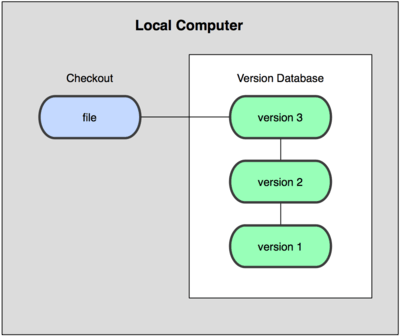
\includegraphics[width=0.5\textwidth]{git/rcs.png}

\end{frame}

\begin{frame}[t]{Централизованные системы контроля версий}
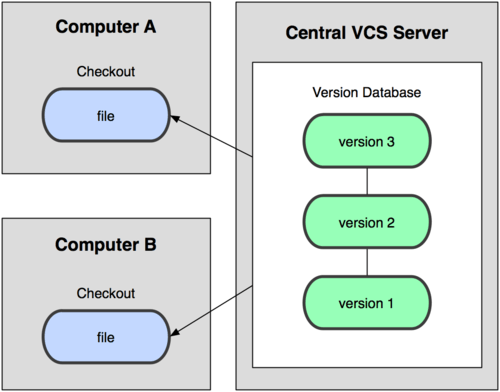
\includegraphics[width=0.5\textwidth]{git/central.png}
\end{frame}

\begin{frame}[t]{Распределённые системы контроля версий}
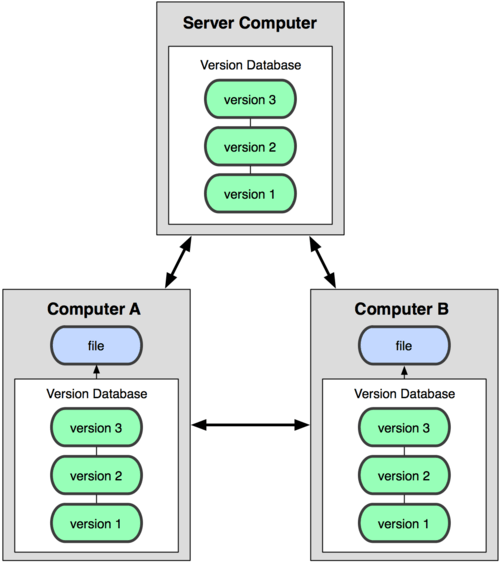
\includegraphics[width=0.5\textwidth]{git/distrib.png}
\end{frame}

\begin{frame}[t]{Git}

Распределённая система управления версиями. 
Проект был создан Линусом Торвальдсом для управления разработкой ядра Linux, первая версия выпущена 7 апреля 2005 года. 
На сегодняшний день его поддерживает Джунио Хамано.

Примерами проектов, использующих Git, являются:
ядро Linux, Android, Drupal, Cairo, GNU Core Utilities, Mesa, Wine, Chromium, Compiz Fusion, FlightGear, jQuery, PHP, NASM, MediaWiki, DokuWiki, Qt и некоторые дистрибутивы Linux 

\url{}

\end{frame}

\begin{frame}[t]{Откуда скачать и установить Git?}


Для Windows --- \url{https://git-for-windows.github.io}

Нажимаете \textbf{Download}, скачивается исполняемый файл, например 
\textbf{Git-2.6.1-64-bit.exe}

Устанавливаете его. 

После установки должна появится в командной строке команда:
\texttt{git}

\end{frame}

 
\subsection{История версий, ветки}
\begin{frame}[t]{Основные команды Git}

\texttt{git init} --- создание нового git-репозитория в текущей папке.
С этого момента в этой папке появляется <<машина времени>> для изменений.
Если вы сделали изменение и зафиксировали его, вы всегда можете откатиться к этой версии.

При успешной инициализации выводится сообщение:
Initialized empty Git repository in FolderName

\texttt{git add} --- добавление файлов в систему контроля версий.
Например: \texttt{git add a.cpp} --- добавить файл a.cpp в СКВ.
\texttt{git add *.cpp} --- добавить все .cpp файлы в СКВ. 
\texttt{git add .} --- добавить все файлы и все каталоги с подкаталогами в СКВ. 

\end{frame}

\subsection{Почитать про Git}
\begin{frame}[t]{Основные команды Git}

\end{frame}
                                         

\end{document}
